\chapter{Řešení Poissonovy rovnice bez okrajových podmínek}

Pokud řešíme Poissonovu rovnici na nekonečné rovině nebo v nekonečném prostoru, pak zde nejsou zadané žádné okrajové podmínky. Začneme odvozením
potenciálu bodového zdroje.

\section{Potenciál v nekonečné rovině bez okrajových podmínek}

Rovnici \eqref{eq:potencial_disku_vne_2} lze využít pro výpočet potenciálu obecného rozložení zdrojů v nekonečné rovině.

Mějme rozdělení hustoty zdrojů \(f(\vect{A})\). Integrováním rovnice \eqref{eq:potencial_disku_vne_2} pak získáme rovnici \eqref{eq:potencial_v_nekonecne_rovine}.

\begin{equation}
\label{eq:potencial_v_nekonecne_rovine}
\varphi(\vect{B}) = \frac{1}{2 \pi} \cdot \int f(\vect{A}) \mathrm{ln} |\vect{A} - \vect{B}| \ d\vect{A}
\end{equation}

\section{Potenciál v nekonečném prostoru bez okrajových podmínek}

Rovnici \eqref{eq:potencial_koule_vne_2} lze využít pro výpočet potenciálu obecného rozložení zdrojů v nekonečném prostoru.

Mějme rozdělení hustoty zdrojů \(f(\vect{A})\). Integrováním rovnice \eqref{eq:potencial_koule_vne_2} pak získáme rovnici \eqref{eq:potencial_v_nekonecnem_prostoru}.

\begin{equation}
\label{eq:potencial_v_nekonecnem_prostoru}
\varphi(\vect{B}) = -\frac{1}{4 \pi} \int \frac{f(\vect{A})}{|\vect{A} - \vect{B}|} \ d\vect{A}
\end{equation}

\subsection{Příklad - vzájemná indukčnost válcových cívek}

Mějme 2 souosé hustě vinuté válcové cívky \(L_1\) a \(L_2\) mající \(N_1\) a \(N_2\) závitů. Cívky jsou na ose mezi souřadnicemi \(x_{11}\) až \(x_{12}\) a \(x_{21}\) až \(x_{22}\) a na poloměrech \(R_{11}\) až \(R_{12}\) a \(R_{21}\) až \(R_{22}\). Cívkou \(L_1\) protéká časově proměnný proud \(i_1(t)\) který v prostoru vyvolá magnetické pole. Toto magnetické pole indukuje v cívce \(L_2\) časově proměnné napětí \(u_2(t)\). Vzájemná indukčnost je definována vztahem \eqref{eq:definice_m}.

\begin{equation}
\label{eq:definice_m}
u_2 = M \cdot \frac{di_1}{dt}
\end{equation}

Pokud bychom chtěli spočítat vlastní indukčnost \(L\), pak stačí zvolit obě cívky shodné, tedy \(L_1 = L_2\).


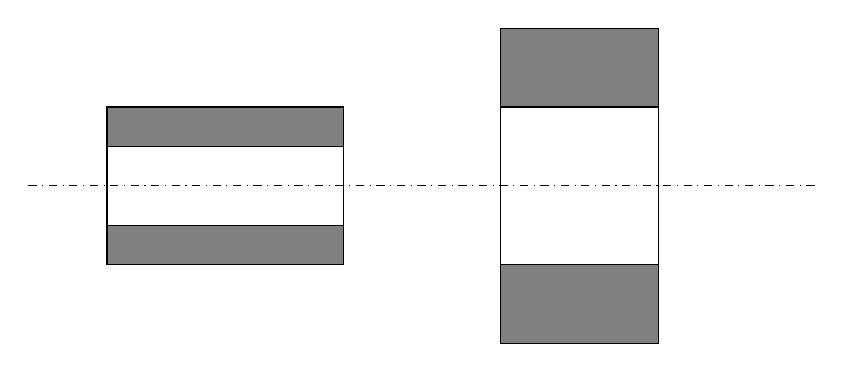
\begin{tikzpicture}
\draw[dashdotted] (0, 0) -- (10, 0);
\draw (1, 0.5) -- (1, -0.5);
\draw (4, 0.5) -- (4, -0.5);
\filldraw[color=black, fill=gray] (1, 0.5) -- (1, 1) -- (4, 1) -- (4, 0.5) -- (1, 0.5);
\filldraw[color=black, fill=gray] (1, -0.5) -- (1, -1) -- (4, -1) -- (4, -0.5) -- (1, -0.5);

\draw (6, 1) -- (6, -1);
\draw (8, 1) -- (8, -1);
\filldraw[color=black, fill=gray] (6, 1) -- (6, 2) -- (8, 2) -- (8, 1) -- (6, 1);
\filldraw[color=black, fill=gray] (6, -1) -- (6, -2) -- (8, -2) -- (8, -1) -- (6, -1);

\end{tikzpicture}

Podle indukčního zákona platí vztah \eqref{eq:indukcni_zakon}.

\begin{equation}
\label{eq:indukcni_zakon}
u_2 = \frac{d\Phi_2}{dt}
\end{equation}

Sloučením vztahů \label{eq:definice_m} a \eqref{eq:indukcni_zakon} získáme vztah \eqref{eq:vypocet_m_obecne}.

\begin{equation}
\label{eq:vypocet_m_obecne}
\begin{split}
M \cdot \frac{di_1}{dt} = \frac{d\Phi_2}{dt} \\
M = \frac{\Phi_2}{i_1} = \frac{\int_{S_2} \vect{B} \cdot {n} ds}{i_1}
\end{split}
\end{equation}

Plocha \(S_2\) je libovolná plocha ohraničená vodičem cívky \(L_2\), pro všechny plochy ohraničené stejným vodičem vyjde integrál stejný.

Cívku \(L_2\) si zjednodušíme jako \(N_2\) kruhových závitů ležících v rovinách kolmých na osu cívky. Protože je cívka hustě vinutá, tak je závitů mnoho a jsou po cívce rovnoměrně rozděleny. Proto si můžeme dovolit namísto počítání jednotlivých závitů zvlášť považovat závity za kontinuum. Závity proložíme kruhy, které jsou kolmé na osu cívky. Proto nás bude zajímat pouze složka indukčnosti rovnoběžná s osou cívky. Tok magnetické indukčnosti kruhy ohraničenými závity cívky nahradíme cirkulací magnetického potenciálu závity. Získáme tak vztah \eqref{eq:aproximace_plochy}. Zde \(\varphi\) je složka magnetického potenciálu rovnoběžná s kruhovým závitem. Díky rotační symetrii úlohy předpokládáme, že tato složka je po celé délce závitu stejná.

Označme plochy poloviny průřezů \(S_1 = (R_{12} - R_{11}) \cdot (L_{12} - L_{11})\) a \(S_2 = (R_{22} - R_{21}) \cdot (L_{22} - L_{21})\).

\begin{equation}
\label{eq:aproximace_plochy}
\begin{split}
M = \int_{S_2} \vect{B} \cdot {n} \ ds = \int_{\partial S_2} \varphi \ dl_2 \approx \\
\frac{N_2}{S_2} \int_{R_{21}}^{R_{22}} \int_{L_{21}}^{L_{22}} \int_{0}^{2 \pi} r_2 \varphi \ d\alpha \ dl_2 \ dr_2 = \\
\frac{N_2}{S_2} \int_{R_{21}}^{R_{22}} \int_{L_{21}}^{L_{22}} 2 \pi r_2 \cdot \varphi(r_2, l_2) \ dl_2 \ dr_2 
\end{split}
\end{equation}

Dále musíme vyjádřit magnetický potenciál \(\varphi\):

\begin{equation}
\label{eq:civky_potencial}
\begin{split}
\varphi(r_2, l_2) = \frac{N_1 \mu}{S_1} \int_{0}^{2 \pi} \int_{R_{11}}^{R_{12}} \int_{L_{11}}^{L_{12}} \frac{r_1}{4 \pi r}  \ dl_1 \ dr_1 \ d \alpha
\end{split}
\end{equation}

\(r\) je vzdálenost elementu cívky \(L_1\) od elementu cívky \(L_2\). Vektor je \(\vect{r} = (l_2 - l_1, r_2 - r_1 \cdot cos \alpha, r1 \cdot sin \alpha)\), proto \(r = \sqrt{(l_2 - l_1)^2 + (r_2 - r_1 \cdot cos \alpha)^2 + r_1^2 \cdot sin^2 \alpha}\).

Indukčnost je tedy

\begin{equation}
\label{eq:indukcnost_1}
\begin{split}
M = \frac{N_1 N_2 \mu}{S_1 S_2} \int_{R_{21}}^{R_{22}} \int_{L_{21}}^{L_{22}} \int_{0}^{2 \pi} \int_{R_{11}}^{R_{12}} \int_{L_{11}}^{L_{12}} \frac{r_1 r_2}{2 r} \ dl_1 \ dr_1 \ d \alpha \ dl_2 \ dr_2
\end{split}
\end{equation}

